\documentclass{article}
\usepackage{graphicx}

\title{Report 6 - Map}
\author{Le Nhu Chu Hiep}

\begin{document}

\maketitle

\section{Algorithm}

For transform to binary image:
\begin{itemize}
\item Setup Image Array
\item Setup threshold value (in 255 scale in this case)
\item Then load each pixel into process
\item Compute average value (int type) from RGB of each pixel
\item Compare value to threshold value
\item If value is higher than threshold, set both RGB of pixel to 255
\item Else set both RGB of pixel to 0
\item Return processed pixel to output
\end{itemize}

\hfill

\noindent For increase brightness of image:
\begin{itemize}
\item Setup Image Array
\item Setup brightness value (in 255 scale in this case)
\item Load each pixel into process
\item Plus both RGB of each pixel with brightness value
\item If RGB value is higher than 255 after plus, set it to 255
\item Return processed pixel to output
\end{itemize}

\hfill

\noindent For blending two images:
\begin{itemize}
\item Load image 1 and image 2 into array
\item Set weight for each image
\item Load each pixel of both 2 images into process
\item With each RGB value, plus value of 2 images multiply with weight and divided by sum of 2 weights
\item Return processed pixel to output
\end{itemize}

\newpage

\section{Result}

\subsection{Text Result}
\begin{verbatim}
USTH ICT Master 2018, Advanced Programming for HPC.
Warming up...
Starting labwork 6
signal 2
labwork 6 GPU binary ellapsed 13.5ms
labwork 6 GPU brighness ellapsed 13.9ms
labwork 6 GPU blending ellapsed 13.5ms
labwork 6 ellapsed 13.6ms
\end{verbatim}

\subsection{Image Result}
The experience used 2 image:

\begin{figure}[h]
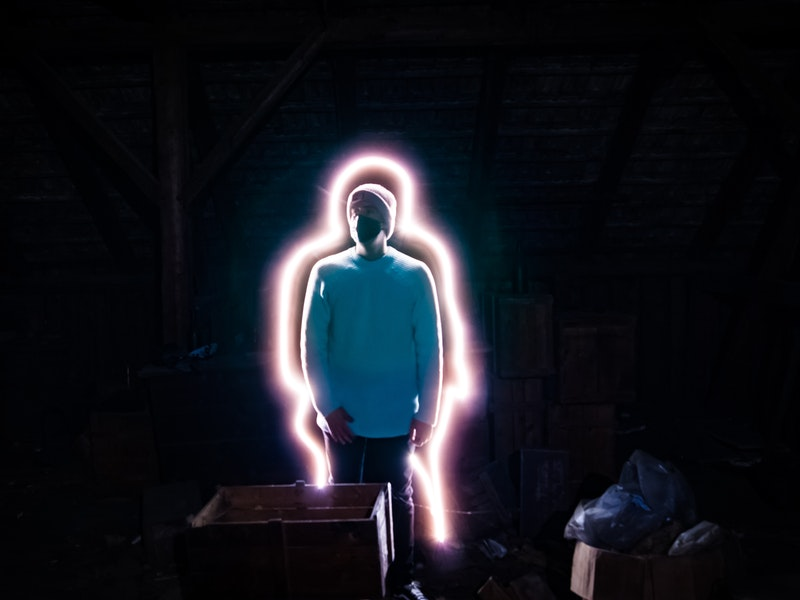
\includegraphics[width=\textwidth]{./labwork/data/ghost.jpeg}
\caption{Main: Ghost JPEG}
\end{figure}

\begin{figure}[h]
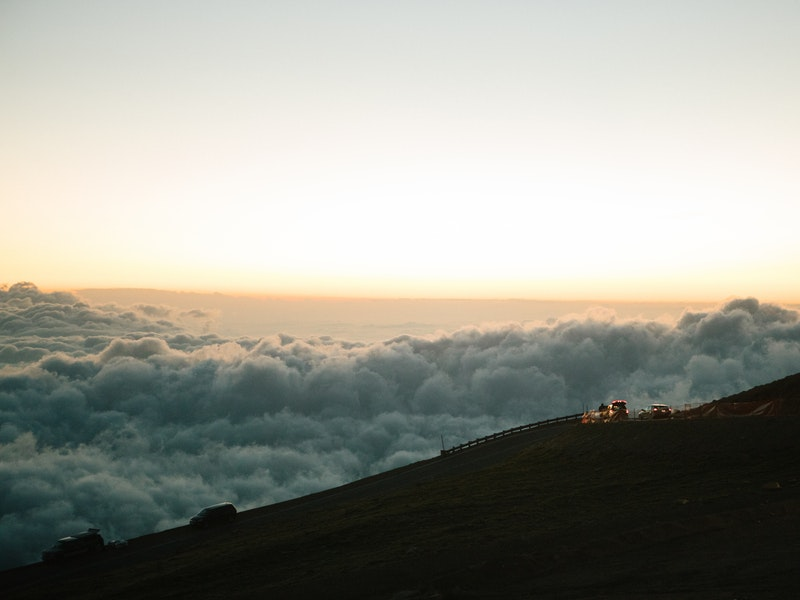
\includegraphics[width=\textwidth]{./labwork/data/cloud.jpeg}
\caption{Secondary: Cloud JPEG}
\end{figure}

Here are output results:

\begin{figure}[h]
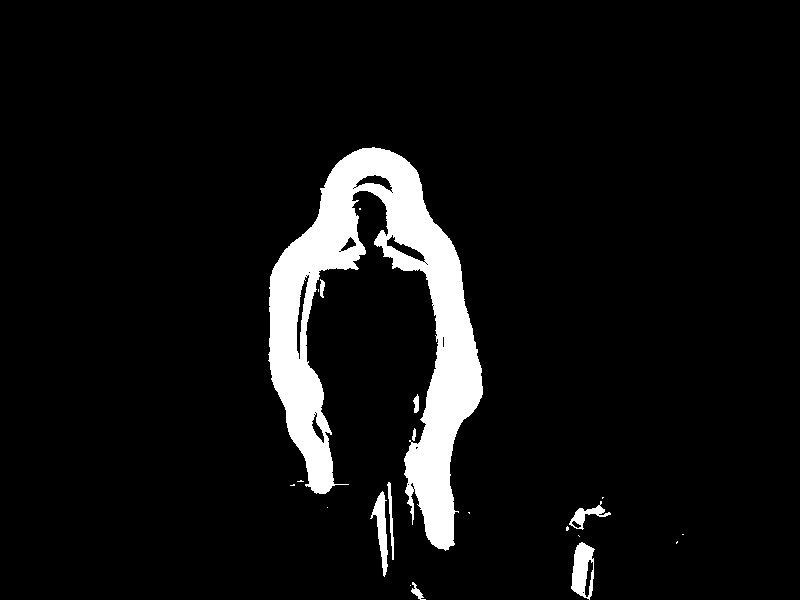
\includegraphics[width=\textwidth]{./labwork6-gpu-out-binary.jpg}
\caption{Binary Result of Ghost JPEG}
\end{figure}

\begin{figure}[h]
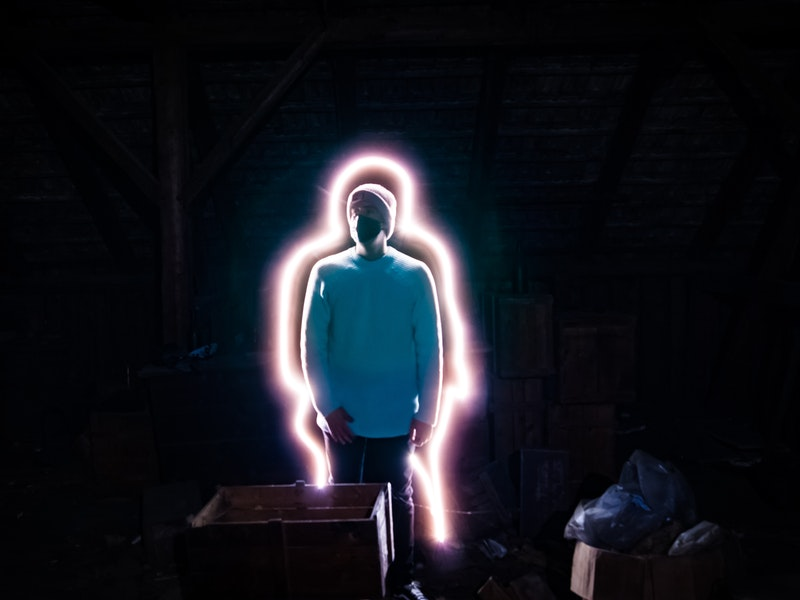
\includegraphics[width=\textwidth]{./labwork/data/ghost.jpeg}
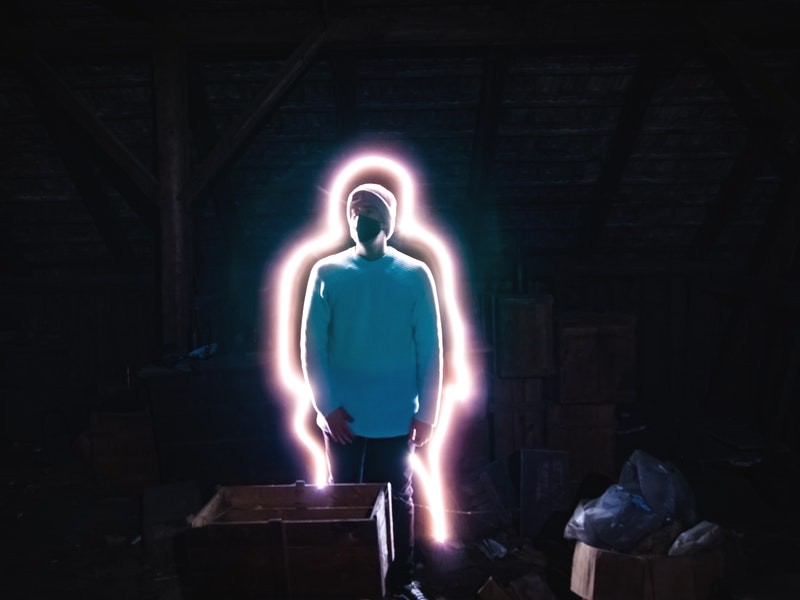
\includegraphics[width=\textwidth]{./labwork6-gpu-out-brightness.jpg}
\caption{Brightness Result of Ghost JPEG}
\end{figure}

\begin{figure}[h]
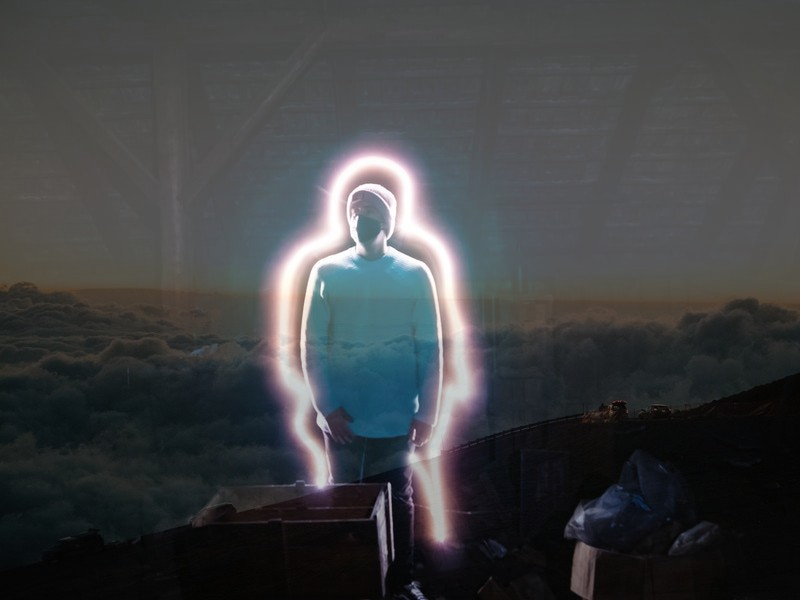
\includegraphics[width=\textwidth]{./labwork6-gpu-out-blending.jpg}
\caption{Blending Result of Ghost and Cloud JPEG}
\end{figure}

\end{document}